\documentclass[10pt]{article}
\usepackage[polish]{babel}
\usepackage[utf8]{inputenc}
\usepackage[T1]{fontenc}
\usepackage{graphicx}
\usepackage[export]{adjustbox}
\graphicspath{ {./images/} }
\usepackage{amsmath}
\usepackage{amsfonts}
\usepackage{amssymb}
\usepackage[version=4]{mhchem}
\usepackage{stmaryrd}
\usepackage{multirow}

\title{Liczba punktów }

\author{}
\date{}


\begin{document}
\maketitle
Arkusz zawiera informacje prawnie chronione do momentu rozpoczęcia egzaminu.\\

\includegraphics[max width=\textwidth, center]{2024_11_21_0c267759828927e3a26dg-01}

\section*{EGZAMIN MATURALNY Z MATEMATYKI \\
 POZIOM PODSTAWOWY}
\begin{enumerate}
  \item Sprawdź, czy arkusz egzaminacyjny zawiera 19 stron (zadania 1-34). Ewentualny brak zgłoś przewodniczącemu zespołu nadzorującego egzamin.
  \item Rozwiązania zadań i odpowiedzi wpisuj w miejscu na to przeznaczonym.
  \item Odpowiedzi do zadań zamkniętych (1-25) przenieś na kartę odpowiedzi, zaznaczając je w części karty przeznaczonej dla zdającego. Zamaluj ■ pola do tego przeznaczone. Błędne zaznaczenie otocz kółkiem i zaznacz właściwe.
  \item Pamiętaj, że pominięcie argumentacji lub istotnych obliczeń w rozwiązaniu zadania otwartego (26-34) może spowodować, że za to rozwiązanie nie otrzymasz pełnej liczby punktów.
  \item Pisz czytelnie i używaj tylko długopisu lub pióra z czarnym tuszem lub atramentem.
  \item Nie używaj korektora, a błędne zapisy wyraźnie przekreśl.
  \item Pamiętaj, że zapisy w brudnopisie nie będą oceniane.
  \item Możesz korzystać z zestawu wzorów matematycznych, cyrkla i linijki oraz kalkulatora.
  \item Na tej stronie oraz na karcie odpowiedzi wpisz swój numer PESEL i przyklej naklejkę z kodem.
  \item Nie wpisuj żadnych znaków w części przeznaczonej dla egzaminatora.
\end{enumerate}

MAJ 2014

Czas pracy:\\
170 minut

do uzyskania: 50

MMA-P1\_1P-142

\section*{ZADANIA ZAMKNIĘTE}
\section*{W zadaniach od 1. do 25. wybierz i zaznacz na karcie odpowiedzi poprawnq odpowiedź.}
\section*{Zadanie 1. (1 pkt)}
Na rysunku przedstawiono geometryczną interpretację jednego z niżej zapisanych układów równań.\\
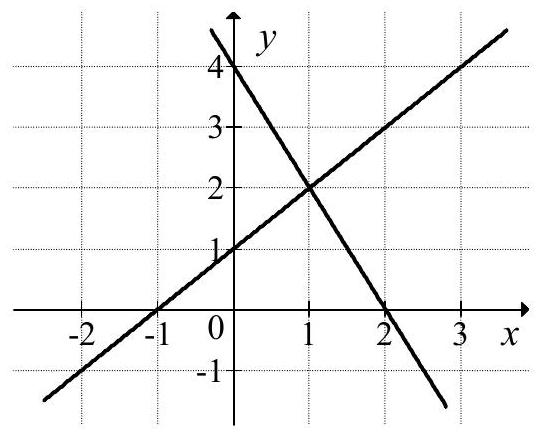
\includegraphics[max width=\textwidth, center]{2024_11_21_0c267759828927e3a26dg-02}

Wskaż ten układ.\\
A. \(\left\{\begin{array}{l}y=x+1 \\ y=-2 x+4\end{array}\right.\)\\
B. \(\left\{\begin{array}{l}y=x-1 \\ y=2 x+4\end{array}\right.\)\\
C. \(\left\{\begin{array}{l}y=x-1 \\ y=-2 x+4\end{array}\right.\)\\
D. \(\left\{\begin{array}{l}y=x+1 \\ y=2 x+4\end{array}\right.\)

\section*{Zadanie 2. (1 pkt)}
Jeżeli liczba 78 jest o \(50 \%\) większa od liczby \(c\), to\\
A. \(c=60\)\\
B. \(c=52\)\\
C. \(c=48\)\\
D. \(c=39\)

\section*{Zadanie 3. (1 pkt)}
Wartość wyrażenia \(\frac{2}{\sqrt{3}-1}-\frac{2}{\sqrt{3}+1}\) jest równa\\
A. -2\\
B. \(-2 \sqrt{3}\)\\
C. 2\\
D. \(2 \sqrt{3}\)

\section*{Zadanie 4.(1 pkt)}
Suma \(\log _{8} 16+1\) jest równa\\
A. 3\\
B. \(\frac{3}{2}\)\\
C. \(\log _{8} 17\)\\
D. \(\frac{7}{3}\)

\section*{Zadanie 5. (1 pkt)}
Wspólnym pierwiastkiem równań \(\left(x^{2}-1\right)(x-10)(x-5)=0\) oraz \(\frac{2 x-10}{x-1}=0\) jest liczba\\
A. -1\\
B. 1\\
C. 5\\
D. 10

\section*{BRUDNOPIS}
\begin{center}

\includegraphics[max width=\textwidth]{2024_11_21_0c267759828927e3a26dg-03}
\end{center}

\section*{Zadanie 6. (1 pkt)}
Funkcja liniowa \(f(x)=\left(m^{2}-4\right) x+2\) jest malejąca, gdy\\
A. \(m \in\{-2,2\}\)\\
B. \(m \in(-2,2)\)\\
C. \(m \in(-\infty,-2)\)\\
D. \(m \in(2,+\infty)\)

\section*{Zadanie 7. (1 pkt)}
Na rysunku przedstawiono fragment wykresu funkcji kwadratowej \(f\).\\
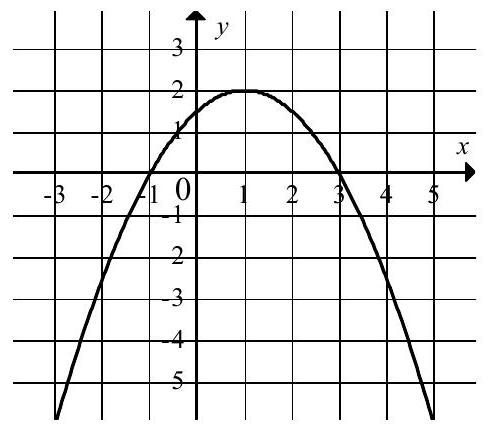
\includegraphics[max width=\textwidth, center]{2024_11_21_0c267759828927e3a26dg-04}

Funkcja \(f\) jest określona wzorem\\
A. \(f(x)=\frac{1}{2}(x+3)(x-1)\)\\
B. \(f(x)=\frac{1}{2}(x-3)(x+1)\)\\
C. \(f(x)=-\frac{1}{2}(x+3)(x-1)\)\\
D. \(f(x)=-\frac{1}{2}(x-3)(x+1)\)

\section*{Zadanie 8. (1 pkt)}
Punkt \(C=(0,2)\) jest wierzchołkiem trapezu \(A B C D\), którego podstawa \(A B\) jest zawarta w prostej o równaniu \(y=2 x-4\). Wskaż równanie prostej zawierającej podstawę \(C D\).\\
A. \(y=\frac{1}{2} x+2\)\\
B. \(y=-2 x+2\)\\
C. \(y=-\frac{1}{2} x+2\)\\
D. \(y=2 x+2\)

\section*{Zadanie 9. (1 pkt)}
Dla każdej liczby \(x\), spełniającej warunek \(-3<x<0\), wyrażenie \(\frac{|x+3|-x+3}{x}\) jest równe\\
A. 2\\
B. 3\\
C. \(-\frac{6}{x}\)\\
D. \(\frac{6}{x}\)

\section*{Zadanie 10. (1 pkt)}
Pierwiastki \(x_{1}, x_{2}\) równania \(2(x+2)(x-2)=0\) spełniają warunek\\
A. \(\frac{1}{x_{1}}+\frac{1}{x_{2}}=-1\)\\
B. \(\frac{1}{x_{1}}+\frac{1}{x_{2}}=0\)\\
C. \(\frac{1}{x_{1}}+\frac{1}{x_{2}}=\frac{1}{4}\)\\
D. \(\frac{1}{x_{1}}+\frac{1}{x_{2}}=\frac{1}{2}\)

\section*{Zadanie 11. (1 pkt)}
Liczby \(2,-1,-4\) są trzema początkowymi wyrazami ciagu arytmetycznego \(\left(a_{n}\right)\), określonego dla liczb naturalnych \(n \geq 1\). Wzór ogólny tego ciagu ma postać\\
A. \(a_{n}=-3 n+5\)\\
B. \(a_{n}=n-3\)\\
C. \(a_{n}=-n+3\)\\
D. \(a_{n}=3 n-5\)

\section*{BRUDNOPIS}
\begin{center}
\begin{tabular}{|c|c|c|c|c|c|c|c|c|c|c|c|c|c|c|c|c|c|c|c|c|c|c|c|}
\hline
 &  &  &  &  &  &  &  &  &  &  &  &  &  &  &  &  &  &  &  &  &  &  &  \\
\hline
 &  &  &  &  &  &  &  &  &  &  &  &  &  &  &  &  &  &  &  &  &  &  &  \\
\hline
 &  &  &  &  &  &  &  &  &  &  &  &  &  &  &  &  &  &  &  &  &  &  &  \\
\hline
 &  &  &  &  &  &  &  &  &  &  &  &  &  &  &  &  &  &  &  &  &  &  &  \\
\hline
 &  &  &  &  &  &  &  &  &  &  &  &  &  &  &  &  &  &  &  &  &  &  &  \\
\hline
 &  &  &  &  &  &  &  &  &  &  &  &  &  &  &  &  &  &  &  &  &  &  &  \\
\hline
 &  &  &  &  &  &  &  &  &  &  &  &  &  &  &  &  &  &  &  &  &  &  &  \\
\hline
 &  &  &  &  &  &  &  &  &  &  &  &  &  &  &  &  &  &  &  &  &  &  &  \\
\hline
 &  &  &  &  &  &  &  &  &  &  &  &  &  &  &  &  &  &  &  &  &  &  &  \\
\hline
 &  &  &  &  &  &  &  &  &  &  &  &  &  &  &  &  &  &  &  &  &  &  &  \\
\hline
 &  &  &  &  &  &  &  &  &  &  &  &  &  &  &  &  &  &  &  &  &  &  &  \\
\hline
 &  &  &  &  &  &  &  &  &  &  &  &  &  &  &  &  &  &  &  &  &  &  &  \\
\hline
 &  &  &  &  &  &  &  &  &  &  &  &  &  &  &  &  &  &  &  &  &  &  &  \\
\hline
 &  &  &  &  &  &  &  &  &  &  &  &  &  &  &  &  &  &  &  &  &  &  &  \\
\hline
 &  &  &  &  &  &  &  &  &  &  &  &  &  &  &  &  &  &  &  &  &  &  &  \\
\hline
 &  &  &  &  &  &  &  &  &  &  &  &  &  &  &  &  &  &  &  &  &  &  &  \\
\hline
 &  &  &  &  &  &  &  &  &  &  &  &  &  &  &  &  &  &  &  &  &  &  &  \\
\hline
 &  &  &  &  &  &  &  &  &  &  &  &  &  &  &  &  &  &  &  &  &  &  &  \\
\hline
 &  &  &  &  &  &  &  &  &  &  &  &  &  &  &  &  &  &  &  &  &  &  &  \\
\hline
 &  &  &  &  &  &  &  &  &  &  &  &  &  &  &  &  &  &  &  &  &  &  &  \\
\hline
 &  &  &  &  &  &  &  &  &  &  &  &  &  &  &  &  &  &  &  &  &  &  &  \\
\hline
 &  &  &  &  &  &  &  &  &  &  &  &  &  &  &  &  &  &  &  &  &  &  &  \\
\hline
 &  &  &  &  &  &  &  &  &  &  &  &  &  &  &  &  &  &  &  &  &  &  &  \\
\hline
 &  &  &  &  &  &  &  &  &  &  &  &  &  &  &  &  &  &  &  &  &  &  &  \\
\hline
 &  &  &  &  &  &  &  &  &  &  &  &  &  &  &  &  &  &  &  &  &  &  &  \\
\hline
 &  &  &  &  &  &  &  &  &  &  &  &  &  &  &  &  &  &  &  &  &  &  &  \\
\hline
 &  &  &  &  &  &  &  &  &  &  &  &  &  &  &  &  &  &  &  &  &  &  &  \\
\hline
 &  &  &  &  &  &  &  &  &  &  &  &  &  &  &  &  &  &  &  &  &  &  &  \\
\hline
 &  &  &  &  &  &  &  &  &  &  &  &  &  &  &  &  &  &  &  &  &  &  &  \\
\hline
 &  &  &  &  &  &  &  &  &  &  &  &  &  &  &  &  &  &  &  &  &  &  &  \\
\hline
 &  &  &  &  &  &  &  &  &  &  &  &  &  &  &  &  &  &  &  &  &  &  &  \\
\hline
 &  &  &  &  &  &  &  &  &  &  &  &  &  &  &  &  &  &  &  &  &  &  &  \\
\hline
 &  &  &  &  &  &  &  &  &  &  &  &  &  &  &  &  &  &  &  &  &  &  &  \\
\hline
 &  &  &  &  &  &  &  &  &  &  &  &  &  &  &  &  &  &  &  &  &  &  &  \\
\hline
 &  &  &  &  &  &  &  &  &  &  &  &  &  &  &  &  &  &  &  &  &  &  &  \\
\hline
 &  &  &  &  &  &  &  &  &  &  &  &  &  &  &  &  &  &  &  &  &  &  &  \\
\hline
 &  &  &  &  &  &  &  &  &  &  &  &  &  &  &  &  &  &  &  &  &  &  &  \\
\hline
 &  &  &  &  &  &  &  &  &  &  &  &  &  &  &  &  &  &  &  &  &  &  &  \\
\hline
 &  &  &  &  &  &  &  &  &  &  &  &  &  &  &  &  &  &  &  &  &  &  &  \\
\hline
 &  &  &  &  &  &  &  &  &  &  &  &  &  &  &  &  &  &  &  &  &  &  &  \\
\hline
 &  &  &  &  &  &  &  &  &  &  &  &  &  &  &  &  &  &  &  &  &  &  &  \\
\hline
 &  &  &  &  &  &  &  &  &  &  &  &  &  &  &  &  &  &  &  &  &  &  &  \\
\hline
 &  &  &  &  &  &  &  &  &  &  &  &  &  &  &  &  &  &  &  &  &  &  &  \\
\hline
 &  &  &  &  &  &  &  &  &  &  &  &  &  &  &  &  &  &  &  &  &  &  &  \\
\hline
 &  &  &  &  &  &  &  &  &  &  &  &  &  &  &  &  &  &  &  &  &  &  &  \\
\hline
\end{tabular}
\end{center}

\section*{Zadanie 12. (1 pkt)}
Jeżeli trójkąty \(A B C\) i \(A^{\prime} B^{\prime} C^{\prime}\) są podobne, a ich pola sa, odpowiednio, równe \(25 \mathrm{~cm}^{2}\) i \(50 \mathrm{~cm}^{2}\), to skala podobieństwa \(\frac{A^{\prime} B^{\prime}}{A B}\) jest równa\\
A. 2\\
B. \(\frac{1}{2}\)\\
C. \(\sqrt{2}\)\\
D. \(\frac{\sqrt{2}}{2}\)

\section*{Zadanie 13. (1 pkt)}
Liczby: \(x-2,6,12\), w podanej kolejności, są trzema kolejnymi wyrazami ciagu geometrycznego. Liczba \(x\) jest równa\\
A. 0\\
B. 2\\
C. 3\\
D. 5

\section*{Zadanie 14. (1 pkt)}
Jeżeli \(\alpha\) jest kątem ostrym oraz \(\operatorname{tg} \alpha=\frac{2}{5}\), to wartość wyrażenia \(\frac{3 \cos \alpha-2 \sin \alpha}{\sin \alpha-5 \cos \alpha}\) jest równa\\
A. \(-\frac{11}{23}\)\\
B. \(\frac{24}{5}\)\\
C. \(-\frac{23}{11}\)\\
D. \(\frac{5}{24}\)

\section*{Zadanie 15. (1 pkt)}
Liczba punktów wspólnych okręgu o równaniu \((x+2)^{2}+(y-3)^{2}=4\) z osiami układu współrzędnych jest równa\\
A. 0\\
B. 1\\
C. 2\\
D. 4

\section*{Zadanie 16. (1 pkt)}
Wysokość trapezu równoramiennego o kącie ostrym \(60^{\circ}\) i ramieniu długości \(2 \sqrt{3}\) jest równa\\
A. \(\sqrt{3}\)\\
B. 3\\
C. \(2 \sqrt{3}\)\\
D. 2

\section*{Zadanie 17. (1 pkt)}
Kąt środkowy oparty na łuku, którego długość jest równa \(\frac{4}{9}\) długości okręgu, ma miarę\\
A. \(160^{\circ}\)\\
B. \(80^{\circ}\)\\
C. \(40^{\circ}\)\\
D. \(20^{\circ}\)

\section*{Zadanie 18. (1 pkt)}
O funkcji liniowej \(f\) wiadomo, że \(f(1)=2\). Do wykresu tej funkcji należy punkt \(P=(-2,3)\). Wzór funkcji \(f\) to\\
A. \(f(x)=-\frac{1}{3} x+\frac{7}{3}\)\\
B. \(f(x)=-\frac{1}{2} x+2\)\\
C. \(f(x)=-3 x+7\)\\
D. \(f(x)=-2 x+4\)

\section*{Zadanie 19. (1 pkt)}
Jeżeli ostrosłup ma 10 krawędzi, to liczba ścian bocznych jest równa\\
A. 5\\
B. 7\\
C. 8\\
D. 10

\section*{BRUDNOPIS}
\begin{center}

\includegraphics[max width=\textwidth]{2024_11_21_0c267759828927e3a26dg-07}
\end{center}

\section*{Zadanie 20. (1 pkt)}
Stożek i walec mają takie same podstawy i równe pola powierzchni bocznych. Wtedy tworząca stożka jest\\
A. sześć razy dłuższa od wysokości walca.\\
B. trzy razy dłuższa od wysokości walca.\\
C. dwa razy dłuższa od wysokości walca.\\
D. równa wysokości walca.

\section*{Zadanie 21. (1 pkt)}
Liczba \(\left(\frac{1}{(\sqrt[3]{729}+\sqrt[4]{256}+2)^{0}}\right)^{-2}\) jest równa\\
A. \(\frac{1}{225}\)\\
B. \(\frac{1}{15}\)\\
C. 1\\
D. 15

\section*{Zadanie 22. (1 pkt)}
Do wykresu funkcji, określonej dla wszystkich liczb rzeczywistych wzorem \(y=-2^{x-2}\), należy punkt\\
A. \(A=(1,-2)\)\\
B. \(B=(2,-1)\)\\
C. \(C=\left(1, \frac{1}{2}\right)\)\\
D. \(\quad D=(4,4)\)

\section*{Zadanie 23. (1 pkt)}
Jeżeli \(A\) jest zdarzeniem losowym, a \(A^{\prime}\)-zdarzeniem przeciwnym do zdarzenia \(A\) oraz zachodzi równość \(P(A)=2 \cdot P\left(A^{\prime}\right)\), to\\
A. \(P(A)=\frac{2}{3}\)\\
B. \(\quad P(A)=\frac{1}{2}\)\\
C. \(P(A)=\frac{1}{3}\)\\
D. \(P(A)=\frac{1}{6}\)

\section*{Zadanie 24. (1 pkt)}
Na ile sposobów można wybrać dwóch graczy spośród 10 zawodników?\\
A. 100\\
B. 90\\
C. 45\\
D. 20

\section*{Zadanie 25. (1 pkt)}
Mediana zestawu danych 2, 12, a, 10, 5, 3 jest równa 7 . Wówczas\\
A. \(a=4\)\\
B. \(a=6\)\\
C. \(a=7\)\\
D. \(a=9\)

\section*{BRUDNOPIS}
\begin{center}
\begin{tabular}{|c|c|c|c|c|c|c|c|c|c|c|c|c|c|c|c|c|c|c|c|c|c|c|c|}
\hline
 &  &  &  &  &  &  &  &  &  &  &  &  &  &  &  &  &  &  &  &  &  &  &  \\
\hline
 &  &  &  &  &  &  &  &  &  &  &  &  &  &  &  &  &  &  &  &  &  &  &  \\
\hline
 &  &  &  &  &  &  &  &  &  &  &  &  &  &  &  &  &  &  &  &  &  &  &  \\
\hline
 &  &  &  &  &  &  &  &  &  &  &  &  &  &  &  &  &  &  &  &  &  &  &  \\
\hline
 &  &  &  &  &  &  &  &  &  &  &  &  &  &  &  &  &  &  &  &  &  &  &  \\
\hline
 &  &  &  &  &  &  &  &  &  &  &  &  &  &  &  &  &  &  &  &  &  &  &  \\
\hline
 &  &  &  &  &  &  &  &  &  &  &  &  &  &  &  &  &  &  &  &  &  &  &  \\
\hline
 &  &  &  &  &  &  &  &  &  &  &  &  &  &  &  &  &  &  &  &  &  &  &  \\
\hline
 &  &  &  &  &  &  &  &  &  &  &  &  &  &  &  &  &  &  &  &  &  &  &  \\
\hline
 &  &  &  &  &  &  &  &  &  &  &  &  &  &  &  &  &  &  &  &  &  &  &  \\
\hline
 &  &  &  &  &  &  &  &  &  &  &  &  &  &  &  &  &  &  &  &  &  &  &  \\
\hline
 &  &  &  &  &  &  &  &  &  &  &  &  &  &  &  &  &  &  &  &  &  &  &  \\
\hline
 &  &  &  &  &  &  &  &  &  &  &  &  &  &  &  &  &  &  &  &  &  &  &  \\
\hline
 &  &  &  &  &  &  &  &  &  &  &  &  &  &  &  &  &  &  &  &  &  &  &  \\
\hline
 &  &  &  &  &  &  &  &  &  &  &  &  &  &  &  &  &  &  &  &  &  &  &  \\
\hline
 &  &  &  &  &  &  &  &  &  &  &  &  &  &  &  &  &  &  &  &  &  &  &  \\
\hline
 &  &  &  &  &  &  &  &  &  &  &  &  &  &  &  &  &  &  &  &  &  &  &  \\
\hline
 &  &  &  &  &  &  &  &  &  &  &  &  &  &  &  &  &  &  &  &  &  &  &  \\
\hline
 &  &  &  &  &  &  &  &  &  &  &  &  &  &  &  &  &  &  &  &  &  &  &  \\
\hline
 &  &  &  &  &  &  &  &  &  &  &  &  &  &  &  &  &  &  &  &  &  &  &  \\
\hline
 &  &  &  &  &  &  &  &  &  &  &  &  &  &  &  &  &  &  &  &  &  &  &  \\
\hline
 &  &  &  &  &  &  &  &  &  &  &  &  &  &  &  &  &  &  &  &  &  &  &  \\
\hline
 &  &  &  &  &  &  &  &  &  &  &  &  &  &  &  &  &  &  &  &  &  &  &  \\
\hline
 &  &  &  &  &  &  &  &  &  &  &  &  &  &  &  &  &  &  &  &  &  &  &  \\
\hline
 &  &  &  &  &  &  &  &  &  &  &  &  &  &  &  &  &  &  &  &  &  &  &  \\
\hline
 &  &  &  &  &  &  &  &  &  &  &  &  &  &  &  &  &  &  &  &  &  &  &  \\
\hline
 &  &  &  &  &  &  &  &  &  &  &  &  &  &  &  &  &  &  &  &  &  &  &  \\
\hline
 &  &  &  &  &  &  &  &  &  &  &  &  &  &  &  &  &  &  &  &  &  &  &  \\
\hline
 &  &  &  &  &  &  &  &  &  &  &  &  &  &  &  &  &  &  &  &  &  &  &  \\
\hline
 &  &  &  &  &  &  &  &  &  &  &  &  &  &  &  &  &  &  &  &  &  &  &  \\
\hline
 &  &  &  &  &  &  &  &  &  &  &  &  &  &  &  &  &  &  &  &  &  &  &  \\
\hline
 &  &  &  &  &  &  &  &  &  &  &  &  &  &  &  &  &  &  &  &  &  &  &  \\
\hline
 &  &  &  &  &  &  &  &  &  &  &  &  &  &  &  &  &  &  &  &  &  &  &  \\
\hline
 &  &  &  &  &  &  &  &  &  &  &  &  &  &  &  &  &  &  &  &  &  &  &  \\
\hline
 &  &  &  &  &  &  &  &  &  &  &  &  &  &  &  &  &  &  &  &  &  &  &  \\
\hline
 & 
\includegraphics[max width=\textwidth]{2024_11_21_0c267759828927e3a26dg-09}
 &  &  &  &  &  &  &  &  &  &  &  &  &  &  &  &  &  &  &  &  &  &  \\
\hline
 & - &  &  &  &  &  &  &  &  &  &  &  &  &  &  &  &  &  &  &  &  &  &  \\
\hline
 & 
\includegraphics[max width=\textwidth]{2024_11_21_0c267759828927e3a26dg-09(2)}
 & 
\includegraphics[max width=\textwidth]{2024_11_21_0c267759828927e3a26dg-09(1)}
 &  &  &  &  &  &  &  &  &  &  &  &  &  &  &  &  &  &  &  &  &  \\
\hline
 & - &  &  &  &  &  &  &  &  &  &  &  &  &  &  &  &  &  &  &  &  &  &  \\
\hline
 & - &  &  &  &  &  &  &  &  &  &  &  &  &  &  &  &  &  &  &  &  &  &  \\
\hline
 & - &  &  &  &  &  &  &  &  &  &  &  &  &  &  &  &  &  &  &  &  &  &  \\
\hline
 &  &  &  &  &  &  &  &  &  &  &  &  &  &  &  &  &  &  &  &  &  &  &  \\
\hline
 & - &  &  &  &  &  &  &  &  &  &  &  &  &  &  &  &  &  &  &  &  &  &  \\
\hline
 &  &  &  &  &  &  &  &  &  &  &  &  &  &  &  &  &  &  &  &  &  &  &  \\
\hline
 &  &  &  &  &  &  &  &  &  &  &  &  &  &  &  &  &  &  &  &  &  &  &  \\
\hline
 &  &  &  &  &  &  &  &  &  &  &  &  &  &  &  &  &  &  &  &  &  &  &  \\
\hline
\end{tabular}
\end{center}

\section*{ZADANIA OTWARTE}
\section*{Rozwiqzania zadań o numerach od 26. do 34. należ̀ zapisać w wyznaczonych miejscach pod treścia zadania.}
Zadanie 26. (2 pkt)\\
Wykresem funkcji kwadratowej \(f(x)=2 x^{2}+b x+c\) jest parabola, której wierzchołkiem jest punkt \(W=(4,0)\). Oblicz wartości współczynników \(b\) i \(c\).\\

\includegraphics[max width=\textwidth, center]{2024_11_21_0c267759828927e3a26dg-10}

Odpowiedź:

\section*{Zadanie 27. (2 pkt)}
Rozwiąż równanie \(9 x^{3}+18 x^{2}-4 x-8=0\).\\

\includegraphics[max width=\textwidth, center]{2024_11_21_0c267759828927e3a26dg-11}

\section*{Odpowiedź:}
\begin{center}
\begin{tabular}{|c|l|c|c|}
\hline
\multirow{2}{*}{\begin{tabular}{l}
Wypelnia \\
egzaminator \\
\end{tabular}} & Nr zadania & 26. & 27. \\
\cline { 2 - 4 }
 & Maks. liczba pkt & \(\mathbf{2}\) & \(\mathbf{2}\) \\
\cline { 2 - 4 }
 & Uzyskana liczba pkt &  &  \\
\hline
\end{tabular}
\end{center}

\section*{Zadanie 28. (2 pkt)}
Udowodnij, że każda liczba całkowita \(k\), która przy dzieleniu przez 7 daje resztę 2 , ma tę własność, że reszta z dzielenia liczby \(3 k^{2}\) przez 7 jest równa 5 .

\begin{center}
\begin{tabular}{|c|c|c|c|c|c|c|c|c|c|c|c|c|c|c|c|c|c|c|c|c|c|c|}
\hline
 &  &  &  &  &  &  &  &  &  &  &  &  &  &  &  &  &  &  &  &  &  &  \\
\hline
 &  &  &  &  &  &  &  &  &  &  &  &  &  &  &  &  &  &  &  &  &  &  \\
\hline
 &  &  &  &  &  &  &  &  &  &  &  &  &  &  &  &  &  &  &  &  &  &  \\
\hline
 &  &  &  &  &  &  &  &  &  &  &  &  &  &  &  &  &  &  &  &  &  &  \\
\hline
 &  &  &  &  &  &  &  &  &  &  &  &  &  &  &  &  &  &  &  &  &  &  \\
\hline
 &  &  &  &  &  &  &  &  &  &  &  &  &  &  &  &  &  &  &  &  &  &  \\
\hline
 &  &  &  &  &  &  &  &  &  &  &  &  &  &  &  &  &  &  &  &  &  &  \\
\hline
 &  &  &  &  &  &  &  &  &  &  &  &  &  &  &  &  &  &  &  &  &  &  \\
\hline
 &  &  &  &  &  &  &  &  &  &  &  &  &  &  &  &  &  &  &  &  &  &  \\
\hline
 &  &  &  &  &  &  &  &  &  &  &  &  &  &  &  &  &  &  &  &  &  &  \\
\hline
 &  &  &  &  &  &  &  &  &  &  &  &  &  &  &  &  &  &  &  &  &  &  \\
\hline
 &  &  &  &  &  &  &  &  &  &  &  &  &  &  &  &  &  &  &  &  &  &  \\
\hline
 &  &  &  &  &  &  &  &  &  &  &  &  &  &  &  &  &  &  &  &  &  &  \\
\hline
 &  &  &  &  &  &  &  &  &  &  &  &  &  &  &  &  &  &  &  &  &  &  \\
\hline
 &  &  &  &  &  &  &  &  &  &  &  &  &  &  &  &  &  &  &  &  &  &  \\
\hline
 &  &  &  &  &  &  &  &  &  &  &  &  &  &  &  &  &  &  &  &  &  &  \\
\hline
 &  &  &  &  &  &  &  &  &  &  &  &  &  &  &  &  &  &  &  &  &  &  \\
\hline
 &  &  &  &  &  &  &  &  &  &  &  &  &  &  &  &  &  &  &  &  &  &  \\
\hline
 &  &  &  &  &  &  &  &  &  &  &  &  &  &  &  &  &  &  &  &  &  &  \\
\hline
 &  &  &  &  &  &  &  &  &  &  &  &  &  &  &  &  &  &  &  &  &  &  \\
\hline
 &  &  &  &  &  &  &  &  &  &  &  &  &  &  &  &  &  &  &  &  &  &  \\
\hline
 &  &  &  &  &  &  &  &  &  &  &  &  &  &  &  &  &  &  &  &  &  &  \\
\hline
 &  &  &  &  &  &  &  &  &  &  &  &  &  &  &  &  &  &  &  &  &  &  \\
\hline
 &  &  &  &  &  &  &  &  &  &  &  &  &  &  &  &  &  &  &  &  &  &  \\
\hline
 &  &  &  &  &  &  &  &  &  &  &  &  &  &  &  &  &  &  &  &  &  &  \\
\hline
 &  &  &  &  &  &  &  &  &  &  &  &  &  &  &  &  &  &  &  &  &  &  \\
\hline
 &  &  &  &  &  &  &  &  &  &  &  &  &  &  &  &  &  &  &  &  &  &  \\
\hline
 &  &  &  &  &  &  &  &  &  &  &  &  &  &  &  &  &  &  &  &  &  &  \\
\hline
 &  &  &  &  &  &  &  &  &  &  &  &  &  &  &  &  &  &  &  &  &  &  \\
\hline
 &  &  &  &  &  &  &  &  &  &  &  &  &  &  &  &  &  &  &  &  &  &  \\
\hline
 &  &  &  &  &  &  &  &  &  &  &  &  &  &  &  &  &  &  &  &  &  &  \\
\hline
 &  &  &  &  &  &  &  &  &  &  &  &  &  &  &  &  &  &  &  &  &  &  \\
\hline
 &  &  &  &  &  &  &  &  &  &  &  &  &  &  &  &  &  &  &  &  &  &  \\
\hline
 &  &  &  &  &  &  &  &  &  &  &  &  &  &  &  &  &  &  &  &  &  &  \\
\hline
 &  &  &  &  &  &  &  &  &  &  &  &  &  &  &  &  &  &  &  &  &  &  \\
\hline
 &  &  &  &  &  &  &  &  &  &  &  &  &  &  &  &  &  &  &  &  &  &  \\
\hline
 &  &  &  &  &  &  &  &  &  &  &  &  &  &  &  &  &  &  &  &  &  &  \\
\hline
 &  &  &  &  &  &  &  &  &  &  &  &  &  &  &  &  &  &  &  &  &  &  \\
\hline
 &  &  &  &  &  &  &  &  &  &  &  &  &  &  &  &  &  &  &  &  &  &  \\
\hline
 &  &  &  &  &  &  &  &  &  &  &  &  &  &  &  &  &  &  &  &  &  &  \\
\hline
 &  &  &  &  &  &  &  &  &  &  &  &  &  &  &  &  &  &  &  &  &  &  \\
\hline
 &  &  &  &  &  &  &  &  &  &  &  &  &  &  &  &  &  &  &  &  &  &  \\
\hline
\end{tabular}
\end{center}

\section*{Zadanie 29. (2 pkt)}
Na rysunku przedstawiono fragment wykresu funkcji \(f\), który powstał w wyniku przesunięcia wykresu funkcji określonej wzorem \(y=\frac{1}{x}\) dla każdej liczby rzeczywistej \(x \neq 0\).\\
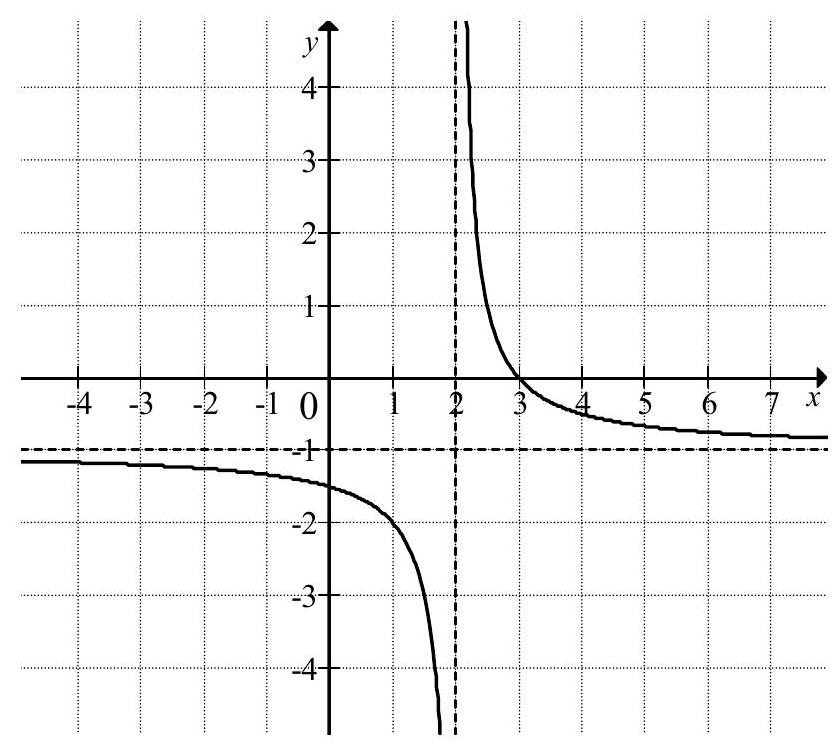
\includegraphics[max width=\textwidth, center]{2024_11_21_0c267759828927e3a26dg-13}\\
a) Odczytaj z wykresu i zapisz zbiór tych wszystkich argumentów, dla których wartości funkcji \(f\) są większe od 0 .\\
b) Podaj miejsce zerowe funkcji \(g\) określonej wzorem \(g(x)=f(x-3)\).\\

\includegraphics[max width=\textwidth, center]{2024_11_21_0c267759828927e3a26dg-13(2)}

Odpowiedź: a)\\
b)\\
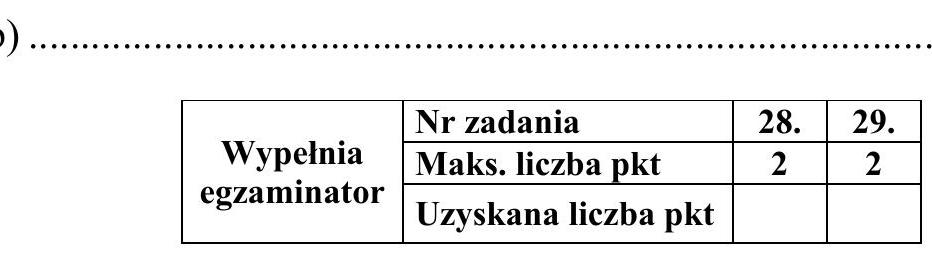
\includegraphics[max width=\textwidth, center]{2024_11_21_0c267759828927e3a26dg-13(1)}

\section*{Zadanie 30. (2 pkt)}
Ze zbioru liczb \(\{1,2,3,4,5,6,7,8\}\) losujemy dwa razy po jednej liczbie ze zwracaniem. Oblicz prawdopodobieństwo zdarzenia \(A\), polegajacego na wylosowaniu liczb, z których pierwsza jest większa od drugiej o 4 lub 6.\\

\includegraphics[max width=\textwidth, center]{2024_11_21_0c267759828927e3a26dg-14}

Odpowiedź:

\section*{Zadanie 31. (2 pkt)}
Środek \(S\) okręgu opisanego na trójkącie równoramiennym \(A B C\), o ramionach \(A C\) i \(B C\), leży wewnątrz tego trójkąta (zobacz rysunek).\\
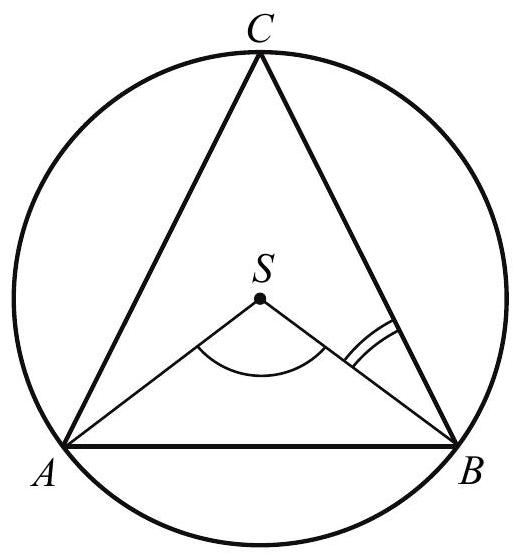
\includegraphics[max width=\textwidth, center]{2024_11_21_0c267759828927e3a26dg-15}

Wykaż, że miara kąta wypukłego \(A S B\) jest cztery razy większa od miary kąta wypukłego SBC.\\

\includegraphics[max width=\textwidth, center]{2024_11_21_0c267759828927e3a26dg-15(1)}

\begin{center}
\begin{tabular}{|c|l|c|c|}
\hline
\multirow{2}{*}{\begin{tabular}{l}
Wypelnia \\
egzaminator \\
\end{tabular}} & Nr zadania & 30. & 31. \\
\cline { 2 - 4 }
 & Maks. liczba pkt & \(\mathbf{2}\) & \(\mathbf{2}\) \\
\cline { 2 - 4 }
 & Uzyskana liczba pkt &  &  \\
\hline
\end{tabular}
\end{center}

\section*{Zadanie 32. (4 pkt)}
Pole powierzchni całkowitej prostopadłościanu jest równe 198. Stosunki długości krawędzi prostopadłościanu wychodzacych z tego samego wierzchołka prostopadłościanu to \(1: 2: 3\). Oblicz długość przekątnej tego prostopadłościanu.\\

\includegraphics[max width=\textwidth, center]{2024_11_21_0c267759828927e3a26dg-16}

Odpowiedź:

\section*{Zadanie 33. (5 pkt)}
Turysta zwiedzał zamek stojacy na wzgórzu. Droga łącząca parking z zamkiem ma długość \(2,1 \mathrm{~km}\). Łączny czas wędrówki turysty z parkingu do zamku i z powrotem, nie licząc czasu poświęconego na zwiedzanie, był równy 1 godzinę i 4 minuty. Oblicz, z jaką średnią prędkością turysta wchodził na wzgórze, jeżeli prędkość ta była o \(1 \frac{\mathrm{~km}}{\mathrm{~h}}\) mniejsza od średniej prędkości, z jaką schodził ze wzgórza.\\

\includegraphics[max width=\textwidth, center]{2024_11_21_0c267759828927e3a26dg-17}

Odpowiedź:

\begin{center}
\begin{tabular}{|c|l|c|c|}
\hline
\multirow{2}{*}{\begin{tabular}{c}
Wypetnia \\
egzaminator \\
\end{tabular}} & Nr zadania & 32. & 33. \\
\cline { 2 - 4 }
 & Maks. liczba pkt & 4 & 5 \\
\cline { 2 - 4 }
 & Uzyskana liczba pkt &  &  \\
\hline
\end{tabular}
\end{center}

\section*{Zadanie 34. (4 pkt)}
Kąt \(C A B\) trójkąta prostokątnego \(A C B\) ma miarę \(30^{\circ}\). Pole kwadratu \(D E F G\), wpisanego w ten trójkąt (zobacz rysunek), jest równe 4. Oblicz pole trójkąta \(A C B\).\\
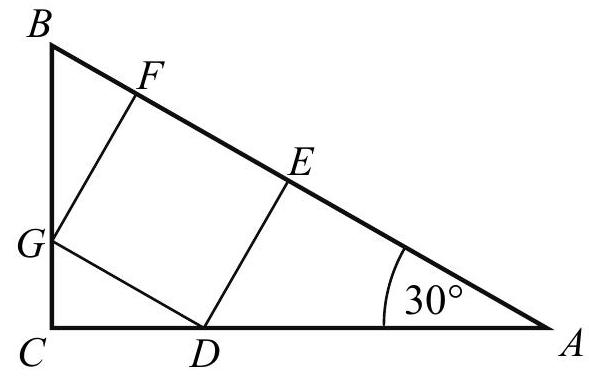
\includegraphics[max width=\textwidth, center]{2024_11_21_0c267759828927e3a26dg-18}\\

\includegraphics[max width=\textwidth, center]{2024_11_21_0c267759828927e3a26dg-18(1)}

Odpowiedź:

\begin{center}
\begin{tabular}{|c|l|c|}
\hline
\multirow{2}{*}{\begin{tabular}{c}
Wypelnia \\
egzaminator \\
\end{tabular}} & Nr zadania & 34. \\
\cline { 2 - 3 }
 & Maks. liczba pkt & 4 \\
\cline { 2 - 3 }
 & Uzyskana liczba pkt &  \\
\hline
\end{tabular}
\end{center}

\section*{BRUDNOPIS}

\end{document}